\documentclass[11pt]{amsart}
\usepackage{amssymb}
\usepackage{tikz}
\usepackage[colorlinks=true, linkcolor=teal, citecolor=teal]{hyperref}

\newtheorem{theorem}{Theorem}[section]
\newtheorem{lemma}[theorem]{Lemma}
\newtheorem{proposition}[theorem]{Proposition}
\theoremstyle{definition}
\newtheorem{definition}[theorem]{Definition}
\theoremstyle{remark}
\newtheorem{remark}[theorem]{Remark}

\newcommand{\Z}{\mathbb{Z}}
\newcommand{\Q}{\mathbb{Q}}
\newcommand{\R}{\mathbb{R}}
\newcommand{\PGL}{\mathrm{PGL}}
\newcommand{\SL}{\mathrm{SL}}

\title{Ping pong in $\PGL_2(\Z[\tfrac12])$}
\author{Nic Brody}
\date{Demo document for the AlphaCentaur talk}

\begin{document}

\begin{abstract}
A two-page example for alphaTeX: the ping-pong lemma, Sanov's free subgroup of
$\SL_2(\Z)$, and why $\PGL_2(\Z[\frac12])$ is discrete only in a product of two
completions.
\end{abstract}

\maketitle

\section{Introduction}\label{sec:intro}

Given finitely many matrices $S \subseteq \PGL_2(\overline{\Q})$, what is the
group $\langle S \rangle$ they generate? The first tool for showing that a group
is free is the ping-pong lemma (Lemma~\ref{lem:pingpong}). Tits used it to show
that a finitely generated linear group either contains a free subgroup of rank
two or is virtually solvable~\cite{tits}.

We give the classical example of Sanov~\cite{sanov} in
Section~\ref{sec:pingpong}, and in Section~\ref{sec:arithmetic} we look at a
group that is not discrete at any single place.

\section{Ping pong}\label{sec:pingpong}

\begin{lemma}[Ping pong]\label{lem:pingpong}
Let $a$ and $b$ act on a set $X$, and let $X_a, X_b \subseteq X$ be disjoint and
nonempty. Suppose $a^n(X_b) \subseteq X_a$ and $b^n(X_a) \subseteq X_b$ for
every $n \neq 0$. Then $\langle a, b \rangle$ is free on $a$ and $b$.
\end{lemma}

\begin{proof}
A nontrivial reduced word in $a$ and $b$ is conjugate to one of the form
$w = a^{n_k} b^{m_{k-1}} \cdots b^{m_1} a^{n_1}$ with every exponent nonzero.
Each letter moves $X_b$ into $X_a$ or $X_a$ into $X_b$ in turn, so
$w(X_b) \subseteq X_a$. Since $X_a \cap X_b = \emptyset$, $w$ is not the
identity.
\end{proof}

\begin{theorem}[Sanov]\label{thm:sanov}
The matrices
\[
  A = \begin{pmatrix} 1 & 2 \\ 0 & 1 \end{pmatrix}, \qquad
  B = \begin{pmatrix} 1 & 0 \\ 2 & 1 \end{pmatrix}
\]
generate a free subgroup of $\SL_2(\Z)$ of rank two.
\end{theorem}

\begin{proof}
Let $\SL_2(\Z)$ act on $\R \cup \{\infty\}$ by M\"obius transformations, and set
$X_A = \{x : |x| > 1\}$ and $X_B = \{x : |x| < 1\}$. If $|x| < 1$ then
$|A^n x| = |x + 2n| > 2|n| - 1 \geq 1$, so $A^n(X_B) \subseteq X_A$. If
$|x| > 1$ then $B^n x = x/(2nx + 1)$ and $|1/B^n x| = |2n + 1/x| > 1$, so
$B^n(X_A) \subseteq X_B$. Apply Lemma~\ref{lem:pingpong}.
\end{proof}

\begin{figure}[ht]
\centering
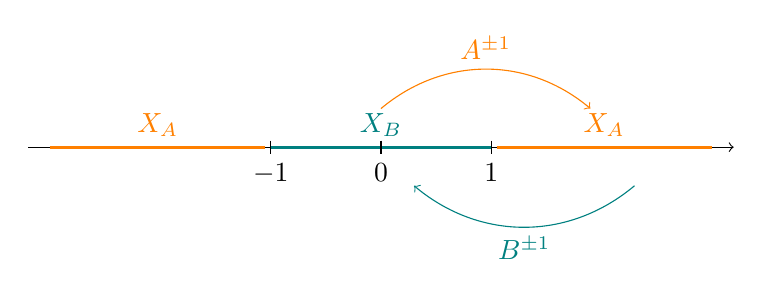
\begin{tikzpicture}[scale=1.4]
  \draw[->] (-3.2,0) -- (3.2,0);
  \draw[very thick, teal] (-1,0) -- (1,0) node[midway, above] {$X_B$};
  \draw[very thick, orange] (-3,0) -- (-1.05,0) node[midway, above] {$X_A$};
  \draw[very thick, orange] (1.05,0) -- (3,0) node[midway, above] {$X_A$};
  \foreach \x in {-1,0,1} \draw (\x,0.06) -- (\x,-0.06) node[below] {$\x$};
  \draw[->, orange] (0,0.35) to[bend left=40] node[above] {$A^{\pm1}$} (1.9,0.35);
  \draw[->, teal] (2.3,-0.35) to[bend left=40] node[below] {$B^{\pm1}$} (0.3,-0.35);
\end{tikzpicture}
\caption{The ping-pong sets for Theorem~\ref{thm:sanov}.}\label{fig:pingpong}
\end{figure}

\section{A group that needs two places}\label{sec:arithmetic}

\begin{proposition}\label{prop:twoplaces}
The group $\Gamma = \PGL_2(\Z[\frac12])$ is not discrete in $\PGL_2(\R)$ or in
$\PGL_2(\Q_2)$, but it is discrete in $\PGL_2(\R) \times \PGL_2(\Q_2)$.
\end{proposition}

\begin{proof}
The ring $\Z[\frac12]$ is dense in $\R$, so the upper triangular unipotent
matrices in $\Gamma$ are not discrete in $\PGL_2(\R)$. In $\PGL_2(\Q_2)$, the
infinite group $\PGL_2(\Z)$ lies in the compact group $\PGL_2(\Z_2)$, so
$\Gamma$ is not discrete there either. Finally, $\Z[\frac12]$ is discrete in
$\R \times \Q_2$, and so $\Gamma$ is discrete in the product; see
\cite[Chapter~II]{serre}, where $\Gamma$ acts on the product of the hyperbolic
plane and the $3$-regular tree.
\end{proof}

\begin{remark}
Proposition~\ref{prop:twoplaces} is why Sanov's group of
Theorem~\ref{thm:sanov} is \emph{geometric} while $\PGL_2(\Z[\frac12])$ is
\emph{arithmetic} in the sense of the Classification Conjecture.
\end{remark}


\begin{thebibliography}{9}
\bibitem{sanov} I.~N. Sanov, \emph{A property of a representation of a free
  group}, Doklady Akad. Nauk SSSR (N.S.) \textbf{57} (1947), 657--659.
\bibitem{serre} J.-P. Serre, \emph{Trees}, Springer-Verlag, Berlin, 1980.
\bibitem{tits} J. Tits, \emph{Free subgroups in linear groups}, J. Algebra
  \textbf{20} (1972), 250--270.
\end{thebibliography}

\end{document}
